% -----------------------------------------
\chapter{Projeto e Desenvolvimento}\label{chp:LABEL_CHP_4}
% -----------------------------------------
Nesta seção são detalhados os passos e decisões tomadas ao decorrer do período de desenvolvimento deste trabalho. São apresentadas as etapas de implementação e integração com outras soluções utilizadas, assim como a execução e comparação dos resultados obtidos.

\section{Casos de uso}
Inicialmente foi desenvolvido o caso de uso expandido do sistema, baseando-se no que foi demonstrado por \citeonline{SOMMERVILE} do modelo UML, como forma tanto de documentação, assim como planejamento do protótipo. Todas as interações do sistema com seus usuários foram pré-determinadas, assim como a definição e organização de requisitos funcionais no sistema dado seu contexto para modelagem do fluxo básico dos eventos diretamente nestes diagramas. O caso de uso, mostra neste contexto o escopo da aplicação, trazendo as principais funcionalidades em que foram desenvolvidas no protótipo, limitando-se a eventos educacionais online. Os cenários de interação entre os atores por meio do caso de uso determinado definem principalmente como deveria ser planejado e até qual ponto pode ser utilizado por cada um deles, respeitando sua hierarquia. A figura \ref{caso_uso_1} demonstra o primeiro caso de uso planejado para o protótipo.

\begin{figure}[H]
    \caption{\label{caso_uso_1}Primeiro caso de uso}
    \vspace{5pt}
    \centering
    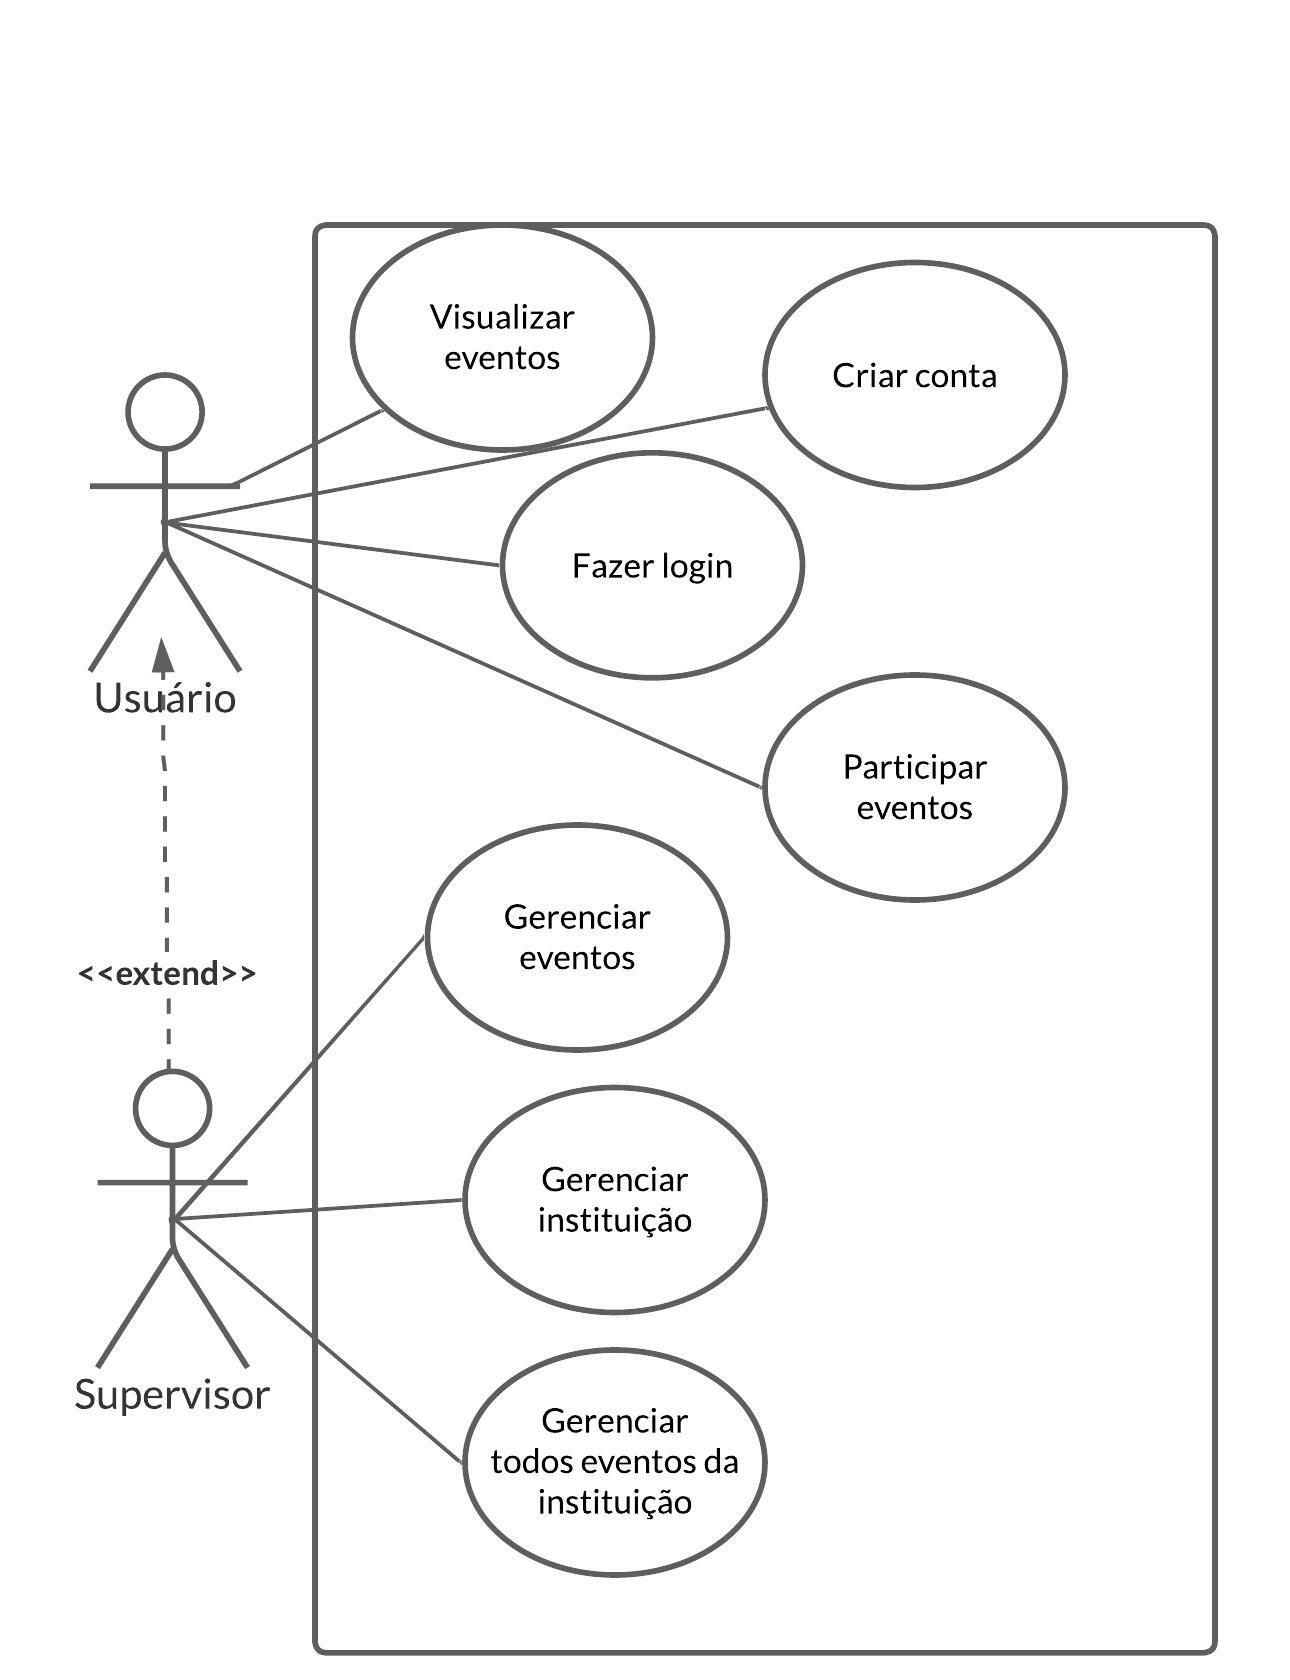
\includegraphics[scale=.6]{Caso de uso TCC1.jpeg}
    \vspace{5pt}
    \legend{Fonte: Próprio autor}
\end{figure}


Com base nesse diagrama, e sua devida explicação, foi possível traçar uma rota de desenvolvimento por meio do processo unificado. No início foi pensado em apenas dois atores, sendo estes um administrador e um usuário comum, como mostra a imagem. Nisto, foram desenvolvidas funcionalidades básicas para estes, contendo a primeira iteração, sem os demais. 

Para a segunda iteração, já há mais atores contando com a inclusão do associado, sendo intermediário entre usuário e supervisor. Além disso, e novas funcionalidades pensadas para a aplicação, sendo estas a gerência da lista de participantes e a gerência dos eventos apenas para determinado usuários (sendo estas relacionadas ao associado) conforme demonstrado na figura \ref{caso_uso_2}.

\begin{figure}[H]
    \caption{\label{caso_uso_2}Segundo caso de uso}
    \vspace{5pt}
    \centering
    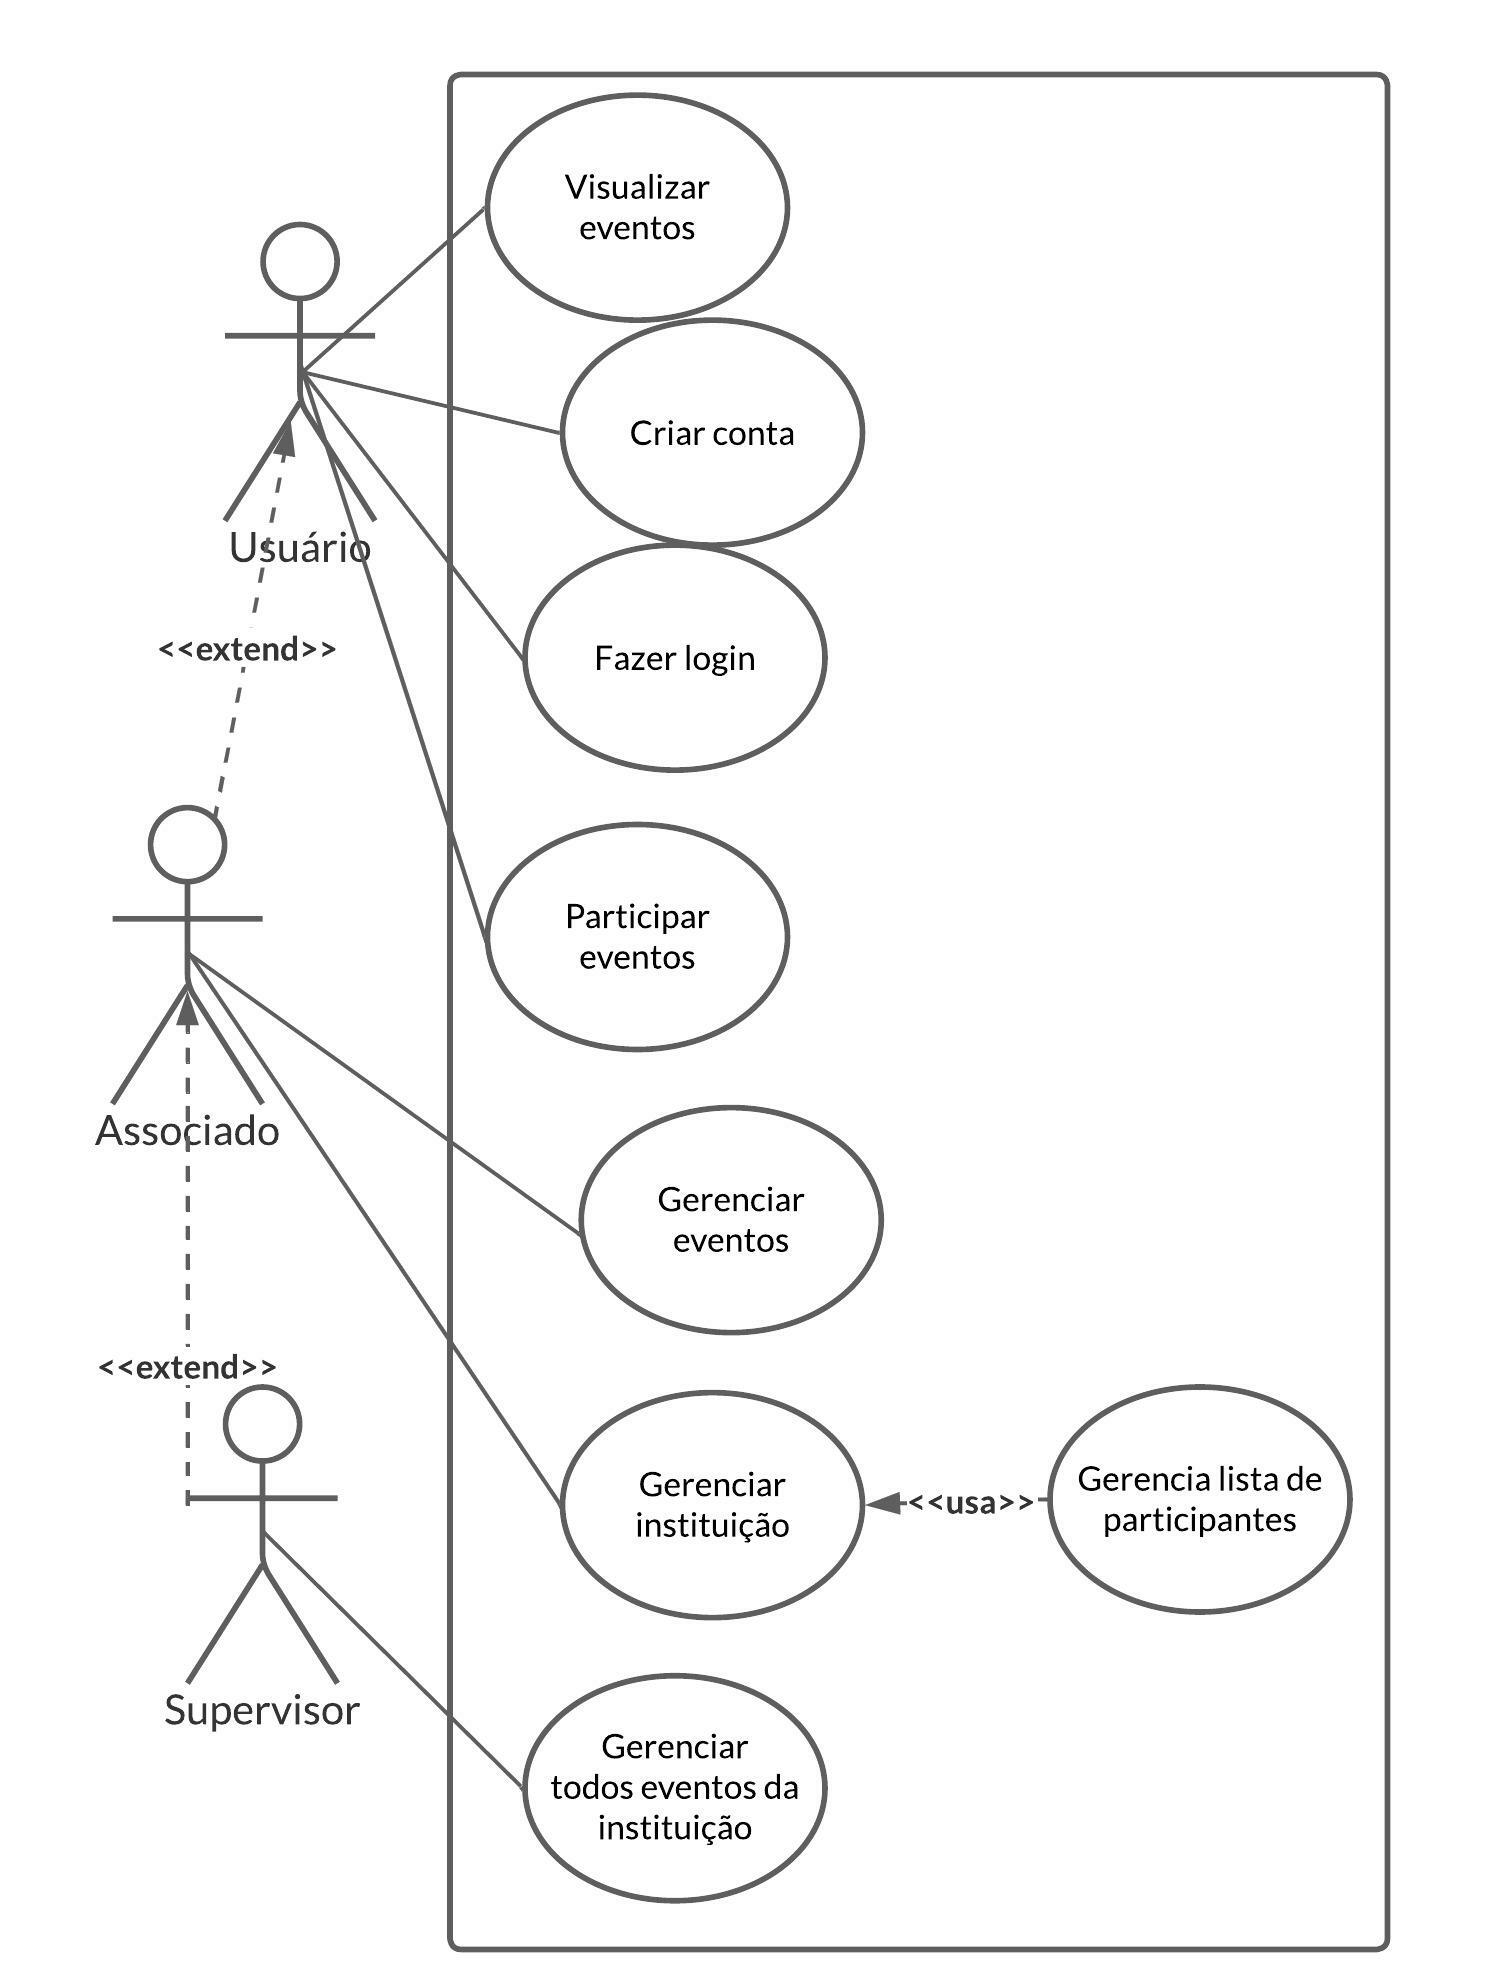
\includegraphics[scale=.7]{Caso de uso TCC2.jpeg}
    \vspace{5pt}
    \legend{Fonte: Próprio autor}
\end{figure}

Na terceira iteração foram identificadas necessidades de atores que não precisavam necessariamente de um \textit{login}, como o visitante, que poderá apenas visualizar os eventos e validar certificados, operações mais simples e que não necessitam de qualquer permissão especial conforme o que é exibido na figura \ref{caso_uso_3}. 

\begin{figure}[H]
    \caption{\label{caso_uso_3}Terceiro caso de uso}
    \vspace{5pt}
    \centering
    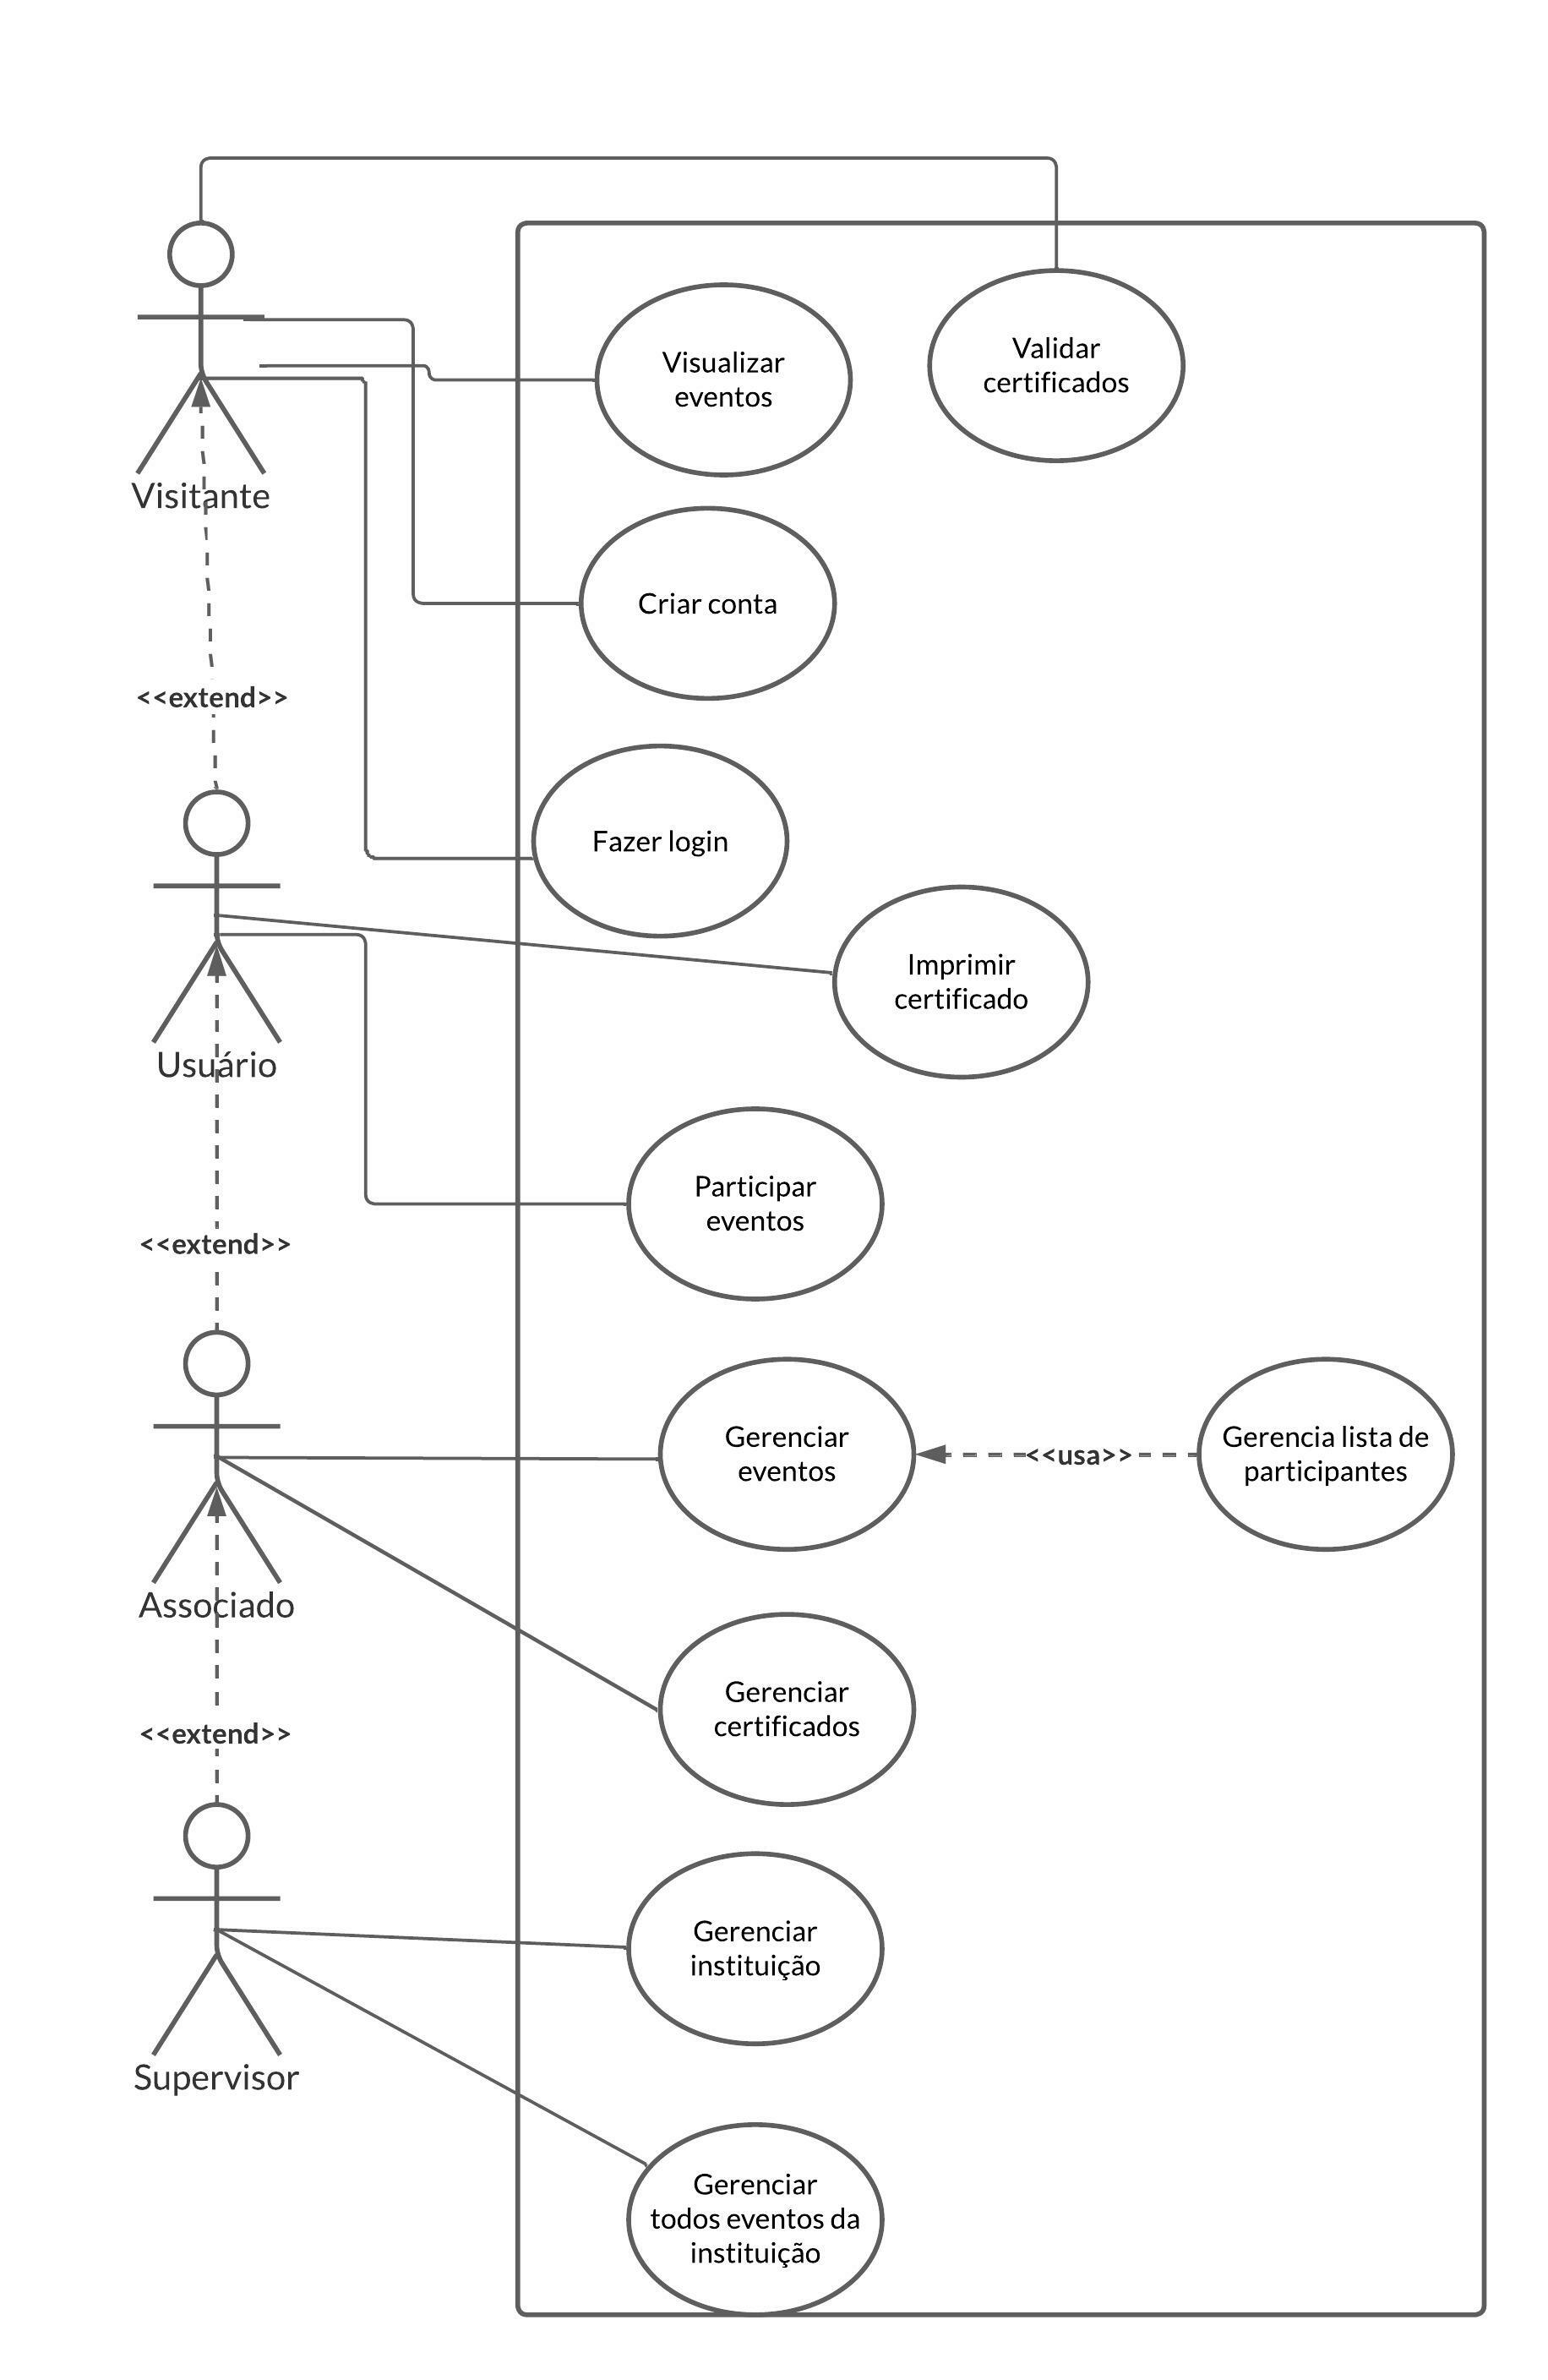
\includegraphics[scale=.7]{Caso de uso TCC3.jpeg}
    \vspace{5pt}
    \legend{Fonte: Próprio autor}
\end{figure}

Na quarta e última iteração até o momento o sistema está mais moldado pensando em diversas funcionalidades, inclusive com o caso de uso expandido, tendo em vista melhor as funcionalidades e seus retornos do sistema para o ator determinado conforme a figura \ref{caso_uso_4}.

\begin{figure}[H]
    \caption{\label{caso_uso_4}Quarto caso de uso}
    \vspace{5pt}
    \centering
    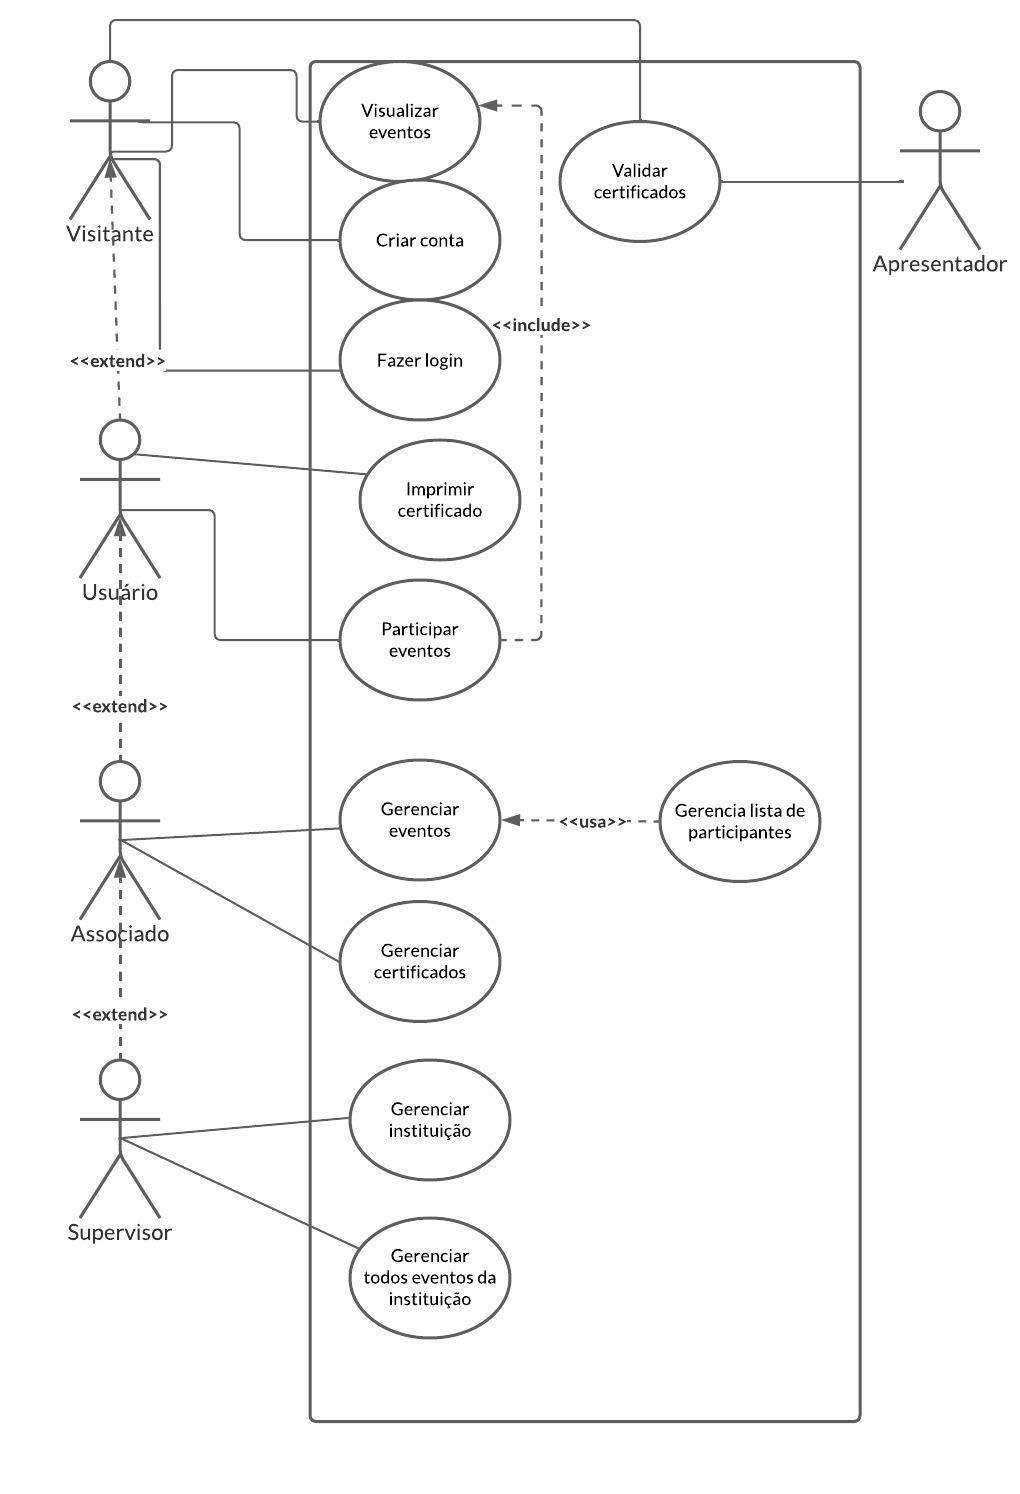
\includegraphics[scale=.7]{Caso de uso TCC4.jpeg}
    \vspace{5pt}
    \legend{Fonte: Próprio autor}
\end{figure}

\subsection{Caso de uso expandido}
Segundo \citeonline{WAZLAWICK}, o caso de uso expandido corresponde ao aprofundamento da análise de requisitos, ou seja, descreve-se mais detalhadamente os passos para cada caso de uso documentado, conforme demonstrado abaixo:

\begin{itemize}
    \item CSU01: visualizar eventos 
        \begin{itemize}
            % \item Pré-condições:
            \item Descrição: O sistema apresenta uma lista de eventos e o usuário pode selecionar um evento para visualização mais detalhada.
            % \item Pós-condições
        \end{itemize}
    \item CSU02: Criar conta
    \begin{itemize}
            \item Descrição: O usuário informa o nome, e-mail, telefone, CPF e senha. O sistema valida as informações digitadas e cria a conta.
            \item Pós-condições: Um e-mail é enviado ao usuário para verificação.
        \end{itemize}
    \item CSU03: Fazer login
        \begin{itemize}
            \item Pré-condições: O usuário deve ter criado a conta anteriormente com o e-mail validado.
            \item Descrição: O usuário informa o e-mail e senha. O sistema valida as informações digitadas e realiza o login.
            \item Pós-condições: O sistema deixa salvo as informações para que, na próxima entrada do usuário, não seja necessário digitar novamente os dados.
            \end{itemize}
    \item CSU04: Imprimir certificado
        \begin{itemize}
            \item Pré-condições: O usuário deve ter participado anteriormente de um evento.
            \item Descrição: O participante ou apresentador geram o arquivo PDF do evento selecionado.
        \end{itemize}
    \item CSU05: Participar eventos
        \begin{itemize}
            \item Pré-condições: O usuário deve ter efetuado o login e selecionado um evento previamente.
            \item Descrição: O participante seleciona as atividades de um determinado evento e participa destas.
            \item Pós-condições: O associado ou supervisor podem selecionar quem foi ao evento para geração do certificado.
        \end{itemize}
    \item CSU06: Gerenciar eventos
        \begin{itemize}
            \item Pré-condições: O usuário deve ter feito login com permissão de associado ou supervisor e selecionar um evento que ainda não ocorreu nenhuma de suas atividades.
            \item Descrição: O usuário pode editar, excluir eventos já cadastrados no sistema. Na edição será possível alterar atividades, descrição e apresentadores.
        \end{itemize}
    \item CSU07: Gerenciar certificados
        \begin{itemize}
            \item Pré-condições: O usuário deve ter efetuado login com permissão de associado ou supervisor.
            \item Descrição: O usuário pode criar, editar ou excluir modelos padrões de certificado. Para criação é necessário que informe a imagem de fundo, banner e assinatura, um título e nome e cargo de quem irá assinar.
            \item Pós-condições: o sistema irá gravar as informações e poderão ser utilizadas para qualquer certificado de evento.
        \end{itemize}
    \item CSU08: Gerenciar instituição
        \begin{itemize}
            \item Pré-condições: O usuário deve ter efetuado login com permissão de supervisor.
            \item Descrição: É possível alterar dados da instituição como seu nome, o supervisor e gerenciar os associados. Ao alterar o supervisor ou adicionar um associado, o sistema verifica se é um usuário válido.
        \end{itemize}
    \item CSU09: Gerenciar todos os eventos da instituição
        \begin{itemize}
            \item Pré-condições: O usuário deve ter efetuado login com permissão de supervisor.
            \item Descrição: O supervisor pode alterar qualquer evento da instituição, sendo ou não criado por seu usuário.
        \end{itemize}
    \item CSU10: Validar certificados
        \begin{itemize}
            \item Descrição: O usuário informa o código de verificação do certificado.
            \item Pós-condições: O sistema retorna se o certificado é válido ou não.
        \end{itemize}
    \item CSU11: Gerencia lista de participantes
        \begin{itemize}
            \item Pré-condições: O usuário deve ter efetuado login com permissão de supervisor ou associado e selecionado um evento.
            \item Descrição: O usuário pode selecionar quem participou do evento, seja participante ou apresentador para gerar um certificado.
            \item Pós-condições: O certificado em formato PDF é enviado ao e-mail dos participantes e apresentadores selecionados.
        \end{itemize}
        
\end{itemize}

\section{Mockups}
Dados os casos de uso, será possível criar um mockup das telas baseado nestas informações. Ou seja, a criação de telas por meio do Figma possibilitou a visualização e alteração do layout de uma forma simplificada antes de serem implementadas de fato. Dito isso, todo o mockup foi pensado para seguir padrões na interface, como, por exemplo, a barra de navegação está presente em todas as páginas a qual o usuário poderá navegar (com exceções apenas da criação de conta e login). E isto facilita a navegação, e mantém a similaridade da aplicação para o usuário final.  

A figura \ref{home_mockup} demonstra como é a ideia da página inicial, que contém uma barra de navegação, um acesso aos eventos, um acesso à criação de eventos e ao perfil. Haverá, no meio da página, um destaque aos últimos eventos cadastrados na plataforma, podendo ser acessados diretamente desta página.
\begin{figure}[H]
    \caption{\label{home_mockup}Mockup da tela inicial}
    \vspace{5pt}
    \centering
    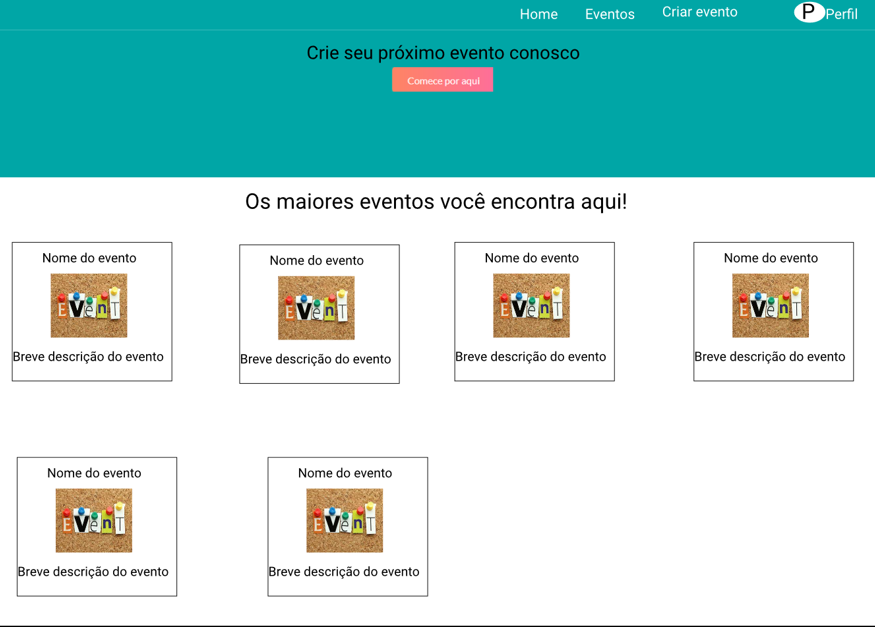
\includegraphics[scale=.4]{home_mockup.png}
    \vspace{5pt}
    \legend{Fonte: Próprio autor}
\end{figure}

Para a página seguinte, a figura \ref{evento_mockup} mostra como é a visualização detalhada de um evento, com sua descrição, imagem e suas atividades cadastradas. Estes detalhes são os compostos especificamente para um evento, mas a barra de navegação citada anteriormente na página inicial estará presente para facilitar a navegação entre páginas.
\begin{figure}[h]
    \caption{\label{evento_mockup}Mockup da tela do evento}
    \vspace{5pt}
    \centering
    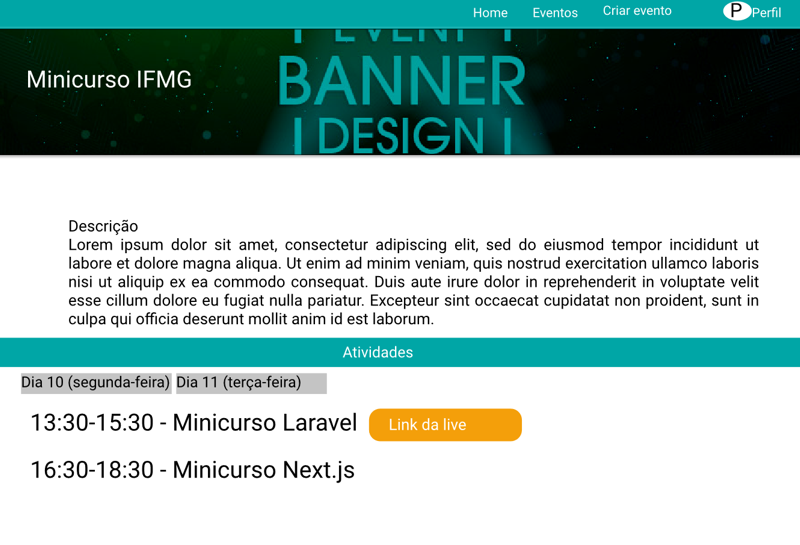
\includegraphics[scale=.4]{evento_mockup.png}
    \vspace{5pt}
    \legend{Fonte: Próprio autor}
\end{figure}

A terceira parte do mockup é a tela de pesquisa de eventos, como mostra a figura \ref{pesquisa_mockup}, que assim como as demais mantém a barra de navegação para facilitar o acesso e possui diversos filtros para os eventos. Estes filtros, definidos por categoria, instituição, data inicial e final e horário inicial e final, foram definidos como os principais para a pesquisa. E ao final da página, percebe-se a paginação, ou seja, caso passe de uma determinada quantidade, serão criadas diversas abas possíveis da mesma pesquisa.
\begin{figure}[H]
    \caption{\label{pesquisa_mockup}Mockup da tela de pesquisa}
    \vspace{5pt}
    \centering
    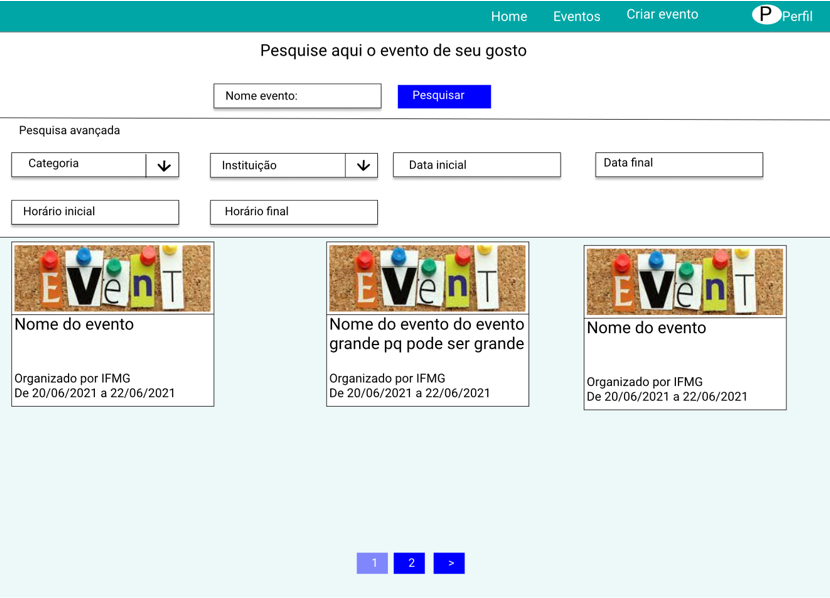
\includegraphics[scale=.4]{pesquisa_mockup.png}
    \vspace{5pt}
    \legend{Fonte: Próprio autor}
\end{figure}

Por fim, a figura \ref{form_mockup}, mostra como serão todos os formulários do sistema, sendo este utilizado conforme a necessidade da tela, como a criação de eventos ou criação de usuário. Isto se deve para melhorar tal interação, tornando padronizado e fazendo com que não seja necessário retrabalho de aprendizagem para cada página contida.
\begin{figure}[H]
    \caption{\label{form_mockup}Mockup da tela de formulário padrão}
    \vspace{5pt}
    \centering
    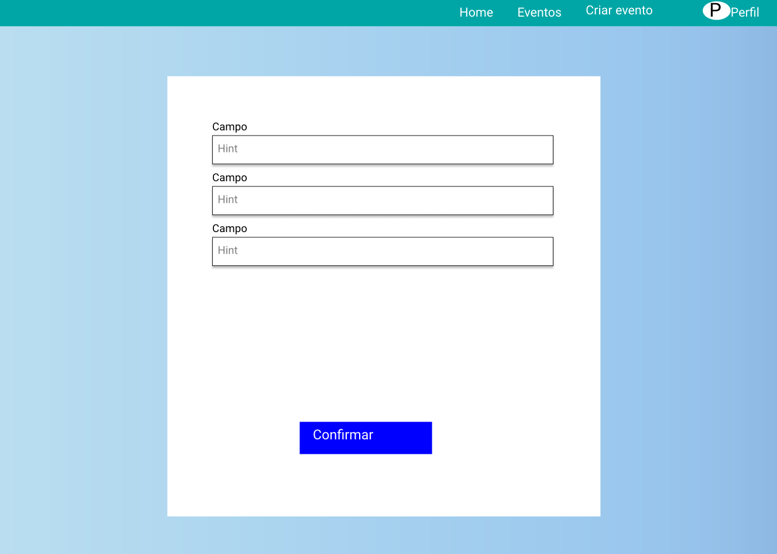
\includegraphics[scale=.4]{form_mockup.png}
    \vspace{5pt}
    \legend{Fonte: Próprio autor}
\end{figure}

Com estas informações sobre a responsabilidade e design de cada tela da aplicação, é possível a criação de maneira estruturada, além de padronizada da interface para o usuário. 

\section{Estruturação}
A estruturação segue um modelo de distribuição vertical, o qual prevê a distinção entre divisão de componentes, neste caso a interface com o usuário e a API, em dois servidores distintos, sendo um alocado na Vercel e outro no Heroku. Mesmo que uma aplicação dependa da outra para funcionar integralmente, são serviços distintos e que melhoram de maneira geral o funcionamento do sistema, visto que tais responsabilidades distintas melhoram o tempo de carregamento de acordo com \citeonline{COULOURIS}. Ou seja, enquanto \textit{backend} persiste os dados e os processa diretamente, respondendo a requisições, o \textit{frontend} fará as requisições recuperando o arquivo JSON gerado e o transformando em uma interface gráfica tangível ao usuário.


\section{Modelo de banco de dados}
Nesta etapa foram criados modelos os quais tiveram embasamento no diagrama de Caso de Uso, assim como nos mockups, visto que deve atender os requisitos predeterminados. Foram criados os modelos conforme figura \ref{modelo_banco}, que determina cada classe do banco de dados feita no Laravel para poder representar os relacionamentos entre as tabelas do MySQL, além de determinar cada atributo das classes. Estes foram feitos com base na figura \ref{models_projeto}, que representa o diagrama de entidade e relacionamento do banco de dados.
\begin{figure}[H]
    \caption{\label{models_projeto}Classes de modelo}
    \vspace{5pt}
    \centering
    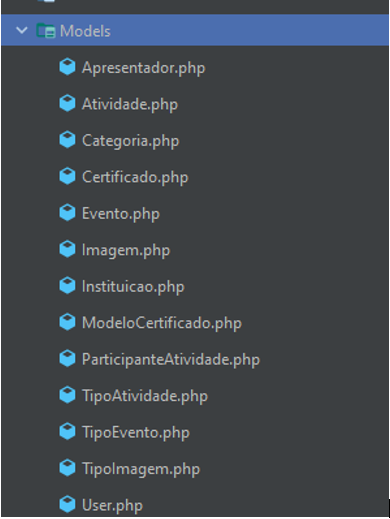
\includegraphics[scale=.8]{models_projeto.png}
    \vspace{5pt}
    \legend{Fonte: Próprio autor}
\end{figure}
\begin{figure}[htbp]
    \caption{\label{modelo_banco}DER do banco de dados}
    \vspace{5pt}
    \centering
    % \includesvg[inkscapelatex=false, width = 100pt]{modelo.svg}
    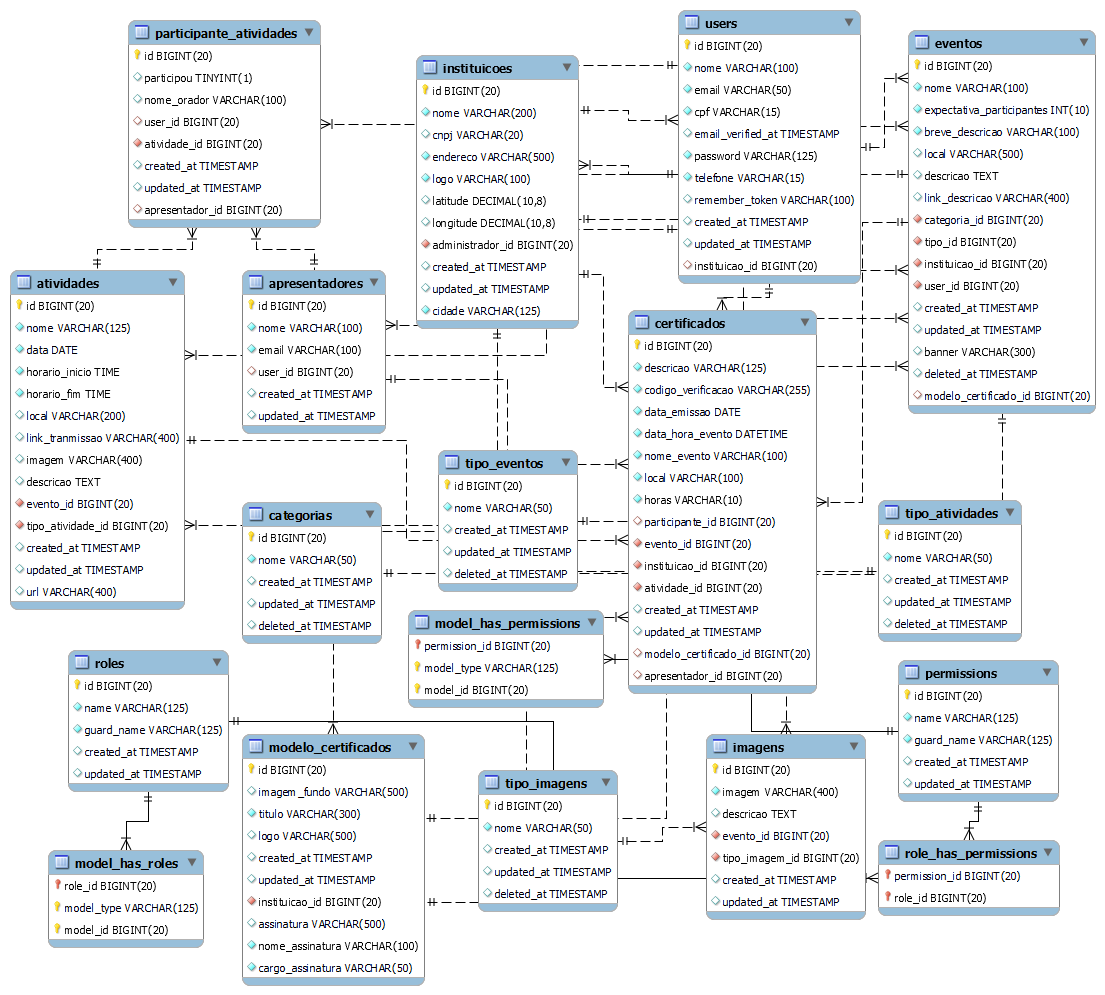
\includegraphics[scale=.5, angle = -90]{modelo.png}
    \vspace{5pt}
    \legend{Fonte: Próprio autor}
\end{figure}
O banco de dados foi planejado criando-se a partir das funcionalidades da aplicação. As tabelas são descritas abaixo:
\begin{itemize}
    \item \textbf{\textit{Users}:} tabela de usuários, com informações básicas do cadastro, contendo nome, e-mail, CPF, senha e telefone. O campo senha é criptografado de modo que tenha segurança ao gravar os dados. Os campos e-mail e CPF devem ser únicos no banco. E há um campo de chave estrangeira, relacionado a instituição, podendo ser nulo, que caso o usuário esteja vinculado a uma instituição, será atribuído o id a ele.
    
    \item \textbf{Instituicoes:} tabela que contém as informações referentes as instituições, tais como o nome, CNPJ, endereço e cidade. O campo CNPJ deve ser único. A chave estrangeira administrador\_id é relacionada ao usuário que criou ou foi transferida a administração da instituição.
    
    \item \textbf{Categorias:} tabela criada com intuito de categorizar os eventos de modo que seja facilitada a busca na aplicação.
    
    \item \textbf{Tipo\_Eventos:} tabela criada com intuito de sub-categorizar os eventos de modo que seja facilitada a busca na aplicação
    
    \item \textbf{Tipo\_Atividades:} tabela criada com intuito de categorizar as atividades de modo que seja facilitada a busca na aplicação.
    
    \item \textbf{Eventos:} tabela que possui os dados do evento, como seu título, expectativa de participantes, banner e uma breve descrição como obrigatórios. Os campos opcionais, como local, descrição podem ser adicionados depois, não sendo obrigatórios. O campo banner é uma URL da imagem armazenada no Firebase. As chaves estrangeiras são definidas pela categoria\_id, tipo\_id (ambas referentes às categorias e tipos escolhidos pelo usuário), instituicao\_id e user\_id (ambas referentes ao usuário que criou o evento) e chave modelo\_certificado\_id (não obrigatória para criação do evento, mas obrigatória para criação dos certificados posteriormente).
    
    \item \textbf{Modelo\_Certificados:} a tabela para os modelos de certificado deve conter os campos de título, nome\_assinatura e cargo\_assinatura como obrigatórios, sendo textos. Os campos de imagem\_fundo, assinatura e logo devem ser preenchidos com as URLs das imagens armazenadas no Firebase. A chave estrangeira instituicao\_id se refere a instituição que criou tal modelo.
    
    \item \textbf{Apresentadores:} os apresentadores podem ser externos à aplicação, então contêm um nome e e-mail. Caso o e-mail seja vinculado a um usuário, será atribuído um id de usuário nesta tabela.
    
    \item \textbf{Tipo\_Imagens:} descreve o tipo de imagem que está no evento, podendo ser banner ou outros.
    
    \item \textbf{Imagens:} tabela que armazena a URL da imagem contida no Firebase, com as chaves estrangeiras de seu tipo e do evento que foi vinculada.
    
    \item \textbf{Atividades:} as atividades são descritas pelo seu nome, a data que irá ocorrer, assim como horário de início e término como obrigatório. Descrição e local podem ser inseridos posteriormente. A URL também pode ser inserida posteriormente, mas é necessário que tenha a URL para que a atividade ocorre, sendo que é com base nela que os participantes entraram. As chaves estrangeiras são: evento\_id, referenciando o evento da atividade e a tipo\_atividade\_id que é sobre o tipo de atividade selecionado.
    
    \item \textbf{Certificados:} esta tabela descreve todas as informações presentes do evento, atividade, data, e as horas da atividade. Deve conter um modelo de certificado para poder se basear as informações. O certificado pode ser para um participante, que deve ser usuário da aplicação, ou um apresentador, podendo este ser externo a aplicação.
    
\end{itemize}

\section{Controllers}
Por meio dos controladores do Laravel, é possível manipular as operações do banco de dados, e para haver uma organização e mantenha o padrão MVC, foram criados controladores específicos para cada modelo, sendo cada um atribuído a responsabilidade do modelo correspondente e essa estruturação pode ser vista na figura \ref{controllers}, a qual demonstra cada um dos controladores.
\begin{figure}[H]
    \caption{\label{controllers}Controladores}
    \vspace{5pt}
    \centering
    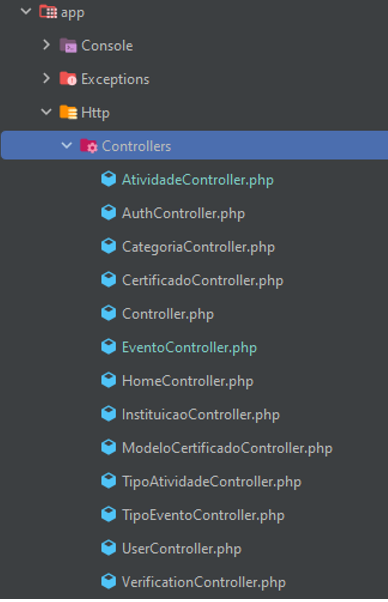
\includegraphics[scale=.5]{controllers.png}
    \vspace{5pt}
    \legend{Fonte: Próprio autor}
\end{figure}

Além disso, por fazerem parte de uma API (explicada com mais detalhes posteriormente), cada operação deve retornar um JSON, com o código de status de retorno do HTTP. No trecho de código, visto no código \ref{orm}, é um exemplo da função a qual recebe uma requisição determinando cada um dos filtros, e então por meio do \textit{eloquent ORM}, realizando a \textit{query} no banco de dados e no fim retornando um JSON com os dados, padronizando, então, a maneira de se receber e retornar os dados.
\begin{lstlisting}[language=PHP, caption = {Exemplo do ORM} \label{orm}]
 public function index(Request $request): JsonResponse {
        $eventos = Evento::query()->with(['atividades' => function ($query) {
            $query->orderBy('data')
            ->orderBy('horario_inicio')
            ->orderBy('horario_fim')
            ->orderBy("nome");
        }, 'categoria', 'instituicao'])
            ->whereHas('atividades')
            ->orderBy('created_at', 'desc');

        if ($request->titulo != null) {
            $queryLower = trim(strtolower($request->titulo));
            $eventos->where(function ($query) use ($queryLower) {
                $query->where(DB::raw('lower(nome)'), 'like', '%' . $queryLower . '%')
                    ->orWhere(DB::raw('lower(breve_descricao)'), 'like', '%' . $queryLower . '%');
            });
        }

        if ($request->cat != null) {
            $eventos->whereRelation('categoria', 'categorias.id', '=', $request->cat);
        }

        if ($request->instituicao != null) {
            $eventos->whereRelation('instituicao', 'instituicoes.id', $request->instituicao);
        }

        if ($request->dataInicio != null) {
            if ($request->dataFim != null) {
                $eventos->whereHas('atividades', function ($q) use ($request) {
                    $q->whereBetween('data', [$request->dataInicio, $request->dataFim]);
                });
            } else {
                $eventos->whereRelation('atividades', 'atividades.data', $request->dataInicio);
            }
        }

        if ($request->horarioInicio != null) {
            $eventos->whereHas('atividades', function ($q) use ($request) {
                $q->whereTime('atividades.horario_inicio', '>=', $request->horarioInicio);
            });
        }

        if ($request->horarioFim != null) {
            $eventos->whereHas('atividades', function ($q) use ($request) {
                $q->whereTime('atividades.horario_fim', '<=', $request->horarioFim);
            });
        }

        return response()->json($eventos->paginate(20));
    }
\end{lstlisting}

Dado o exemplo da busca e seus filtros, a validação de dados na inserção e atualização de dados é essencial para não haver dados inseridos de maneira indevida e que haja um padrão nas requisições. Isto tudo é feito diretamente no Laravel, que validará antes mesmo do banco de dados e retornará caso haja algum erro.

\section{Operações API}
A API foi feita no Laravel, respeitando os padrões estabelecidos pela interface REST. Ou seja, por meio de requisições HTTP do tipo GET, POST e DELETE é possível acessar todas as rotas do \textit{backend}. Em diversas destas não será possível acessar sem que haja uma autenticação feita por meio do JWT, que irá validar se há permissão de acesso, e isto determina caso o usuário esteja logado, assim como seu nível de acesso dentro de sua hierarquia. 

As rotas foram criadas em grupos para atenderem as necessidades e criar-se uma organização para cada requisição, então foram organizadas, conforme o código \ref{rotas_laravel}. Este demonstra cada um dos agrupamentos, sendo estes aqueles que contém todas as rotas para modelos, assim como para determinadas funcionalidades do sistema. O grupo de eventos tem todas as rotas pertencentes a eventos  e conforme pode ser visualizado possuem autenticação e validação do que pode ser escrito na URL para poder ser acessada devidamente. 

\begin{lstlisting}[language=PHP, caption = {Grupo de rotas} \label{rotas_laravel}]
 Route::group(["prefix" => "eventos"], function () {
    Route::get("/", [EventoController::class, 'index']);
    Route::get("/{id}", [EventoController::class, 'show'])->where('id', '[0-9]+');
    Route::get("/categorias/{id}", [EventoController::class, 'porCategoria'])->where('id', '[0-9]+');

    Route::get('/user', [EventoController::class, 'eventos_participados'])->middleware('role:usuario');
    Route::post("/ingressos", [EventoController::class, 'compraIngresso'])->middleware('role:usuario');
    Route::get('/{id}/user/atividades', [EventoController::class, 'atividades_participadas'])->middleware('role:usuario');

    Route::get("/criados", [EventoController::class, 'eventos_criados'])->can('gerenciar_evento');
    Route::post("/store", [EventoController::class, 'store'])->can('gerenciar_evento');
    Route::post("/update/{id}", [EventoController::class, 'update'])->can('gerenciar_evento');
    Route::delete("/{id}", [EventoController::class, 'destroy'])->can('gerenciar_evento');
    Route::post("/{id}/uploadImagens", [EventoController::class, 'upload_imagens'])->can('gerenciar_evento')->where('id', '[0-9]+');
})
\end{lstlisting}

\section{Componentes}
Diferentemente do \textit{webservice} criado no Laravel, a estruturação do \textit{frontend} no Next.js é feito por meio de componentes, e por utilizar o Typescript, há a tipagem em variáveis que auxilia o desenvolvedor nos parâmetros a serem passados entre os componentes do projeto. Na figura \ref{estrutura_next} é possível observar a estruturação geral do projeto, dividido em componentes, páginas, imagens, tipos, utilitários e a configuração do Firebase.
\begin{figure}[H]
    \caption{\label{estrutura_next}Estrutura do projeto do Next.js}
    \vspace{5pt}
    \centering
    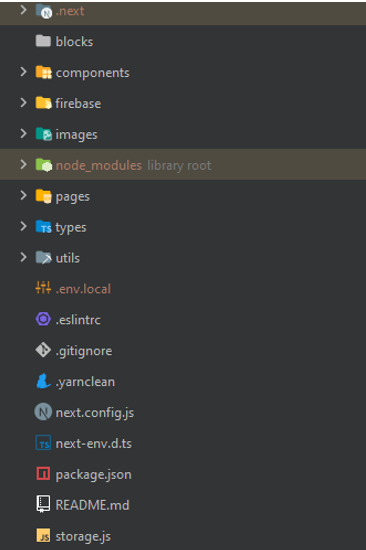
\includegraphics[scale=.45]{estrutura_next.png}
    \vspace{5pt}
    \legend{Fonte: Próprio autor}
\end{figure}

Por meio dos componentes, mostrados na estrutura da figura \ref{componentes} é possível a reutilização do código-fonte para diversos layouts, como, por exemplo, o componente NavBar, o qual é utilizado em diversas páginas, tornando-as padronizadas. Com isto, cada componente, também, terá seu estilo por meio de um arquivo de módulo do CSS, que estende os estilos globais, podendo sobrepô-los. Portanto, cada componente terá sua finalidade pré-definida, podendo ser reutilizada caso sirva o propósito.

\begin{figure}[H]
    \caption{\label{componentes}Estrutura dos componentes}
    \vspace{5pt}
    \centering
    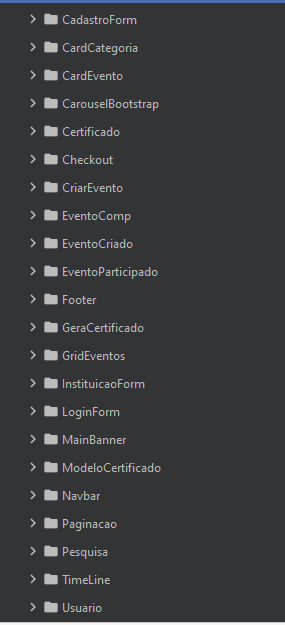
\includegraphics[scale=.45]{componentes.png}
    \vspace{5pt}
    \legend{Fonte: Próprio autor}
\end{figure}

\section{Rotas Next.js}
Em relação às rotas, serão as páginas a serem acessadas pelo usuário. Dito isso, estas deverão validar, caso necessário, se o usuário está logado por meio de uma requisição ao \textit{backend}. Além disso, estas devem requisitar diversas informações para poderem ser exibidas nas páginas e terem os dados necessários preenchidos de cada componente. Conforme estruturação presente na figura \ref{pages}, cada página tem seu nome e sua estruturação interna, podendo ter sub-rotas, que serão chamadas dentro da pasta. Esta regra vale para todas as pastas presentes, com exceção das 404 (a qual está destinada a páginas não encontradas, ou seja, caso seja digitada uma \textit{url} dentro do domínio que não seja pertencente a esta lista, irá a chamar, visto que é uma página customizada) e a 403 (que determina um recurso não possível de ser acessado para determinado usuário).
\begin{figure}[H]
    \caption{\label{pages}Estruturação de páginas no Next.js}
    \vspace{5pt}
    \centering
    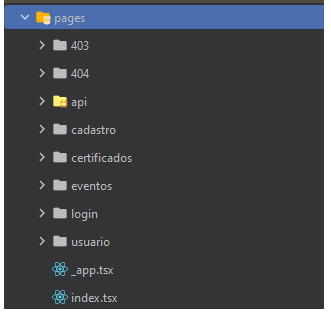
\includegraphics[scale=.6]{pages.png}
    \vspace{5pt}
    \legend{Fonte: Próprio autor}
\end{figure}

\section{Renderização das páginas}
Dentro das páginas da aplicação, diretamente do Next.js, foram utilizadas ambas as implementações de pré-renderização presentes no framework. Em páginas que podem ter cache, como, por exemplo, as páginas individuais de cada evento, principalmente por conterem diversas imagens, além de não necessariamente precisarem estar sendo constantemente atualizadas, sendo estas geradas em tempo de compilação, e tendo em vista que o evento nem seja editado, foi utilizado o método de \textit{Static Generation} com \textit{Incremental Static Regeneration}. Ou seja, por todas as páginas serem baseadas nos mesmos componentes, tendo sua diferença apenas os dados requisitados, foi criado um cache para cada um, gerando uma página HTML com um JSON de dados, para cada uma das páginas. Isto faz com que o acesso seja mais rápido, e o cache é de um minuto, ou seja, a cada um minuto se o evento for editado e caso haja uma requisição, a página será gerada novamente com base no que foi atualizado em cada uma das páginas desta rota dinâmica.

Há também a outra implementação de pré-renderização, sendo a \textit{Server-side rendering}, utilizada em páginas, como a de pesquisa dos eventos. A sua utilização se deve ao fato de que esta deve ser geradas constantemente baseada nos filtros que o usuário irá fazer dada a sua necessidade. A página é mais lenta em relação a uma geração estática, porém todo o processamento fica no servidor que está hospedada a aplicação, deixando com o navegador do usuário final apenas com o HTML gerado em tempo de execução dada essa frequência de atualização desta página, por exemplo.
